\DiaryEntry{Agile Project Management with Scrum (Ken Schwaber)}{2021-09-30}{General}

Taken from \cite{schwaber2004agile}.

\subsection{Introduction}

Complex problems are those that behave unpredictably. Not only are these problems unpredictable, but even the ways in which they will prove unpredictable are impossible to predict.

Much of our society is based on processes that work only because their degree of imprecision is acceptable. What happens when we are building something that requires a degree of precision higher than that obtainable through averaging? What happens if any process that we devise for building cars is too imprecise for our customers, and we need to increase the level of precision? In those cases, we have to guide the process step by step, ensuring that the process converges on an acceptable degree of precision. In cases where convergence doesn’t occur, we have to make adaptations to bring the process back into the range of acceptable precision levels. Laying out a process that repeatably will produce acceptable quality output is called \emph{defined process control}. When defined process control cannot be achieved because of the complexity of the intermediate activities, something called \emph{empirical process control} has to be employed.

We use defined processes whenever possible because with them we can crank up unattended production to such a quantity that the output can be priced as a commodity. However, if the commodity is of such unacceptable quality as to be unusable, the rework is too great to make the price acceptable, or the cost of unacceptably low yields is too high, we have to turn to and accept the higher costs of empirical process control. In the long run, making successful products the first time using empirical process control turns out to be much cheaper than reworking unsuccessful products using defined process control. There are three legs that hold up every implementation of empirical process control: \emph{visibility, inspection, and adaptation}.

Visibility means that those aspects of the process that affect the outcome must be visible to those controlling the process. Not only must these aspects be visible, but what is visible must also be true. There is no room for deceiving appearances in empirical process control. What does it mean, for example, when someone says that certain functionality is labeled “done”? In software development, asserting that functionality is done might lead someone to assume that it is cleanly coded, refactored, unit-tested, built, and acceptance-tested. Someone else might assume that the code has only been built. It doesn’t matter whether it is visible that this functionality is done if no one can agree what the word “done” means.

The second leg is inspection. The various aspects of the process must be inspected frequently enough that unacceptable variances in the process can be detected. The frequency of inspection has to take into consideration that processes are changed by the very act of inspection. Interestingly, the required frequency of inspection often exceeds the tolerance to inspection of the process. Fortunately, this isn’t usually true in software development. The other factor in inspection is the inspector, who must possess the skills to assess what he or she is inspecting.

The third leg of empirical process control is adaptation. If the inspector determines from the inspection that one or more aspects of the process are out- side acceptable limits and that the resulting product will be unacceptable, the inspector must adjust the process or the material being processed. The adjust- ment must be made as quickly as possible to minimize further deviation.

\subsection{Scrum Process}

Scrum hangs all of its practices on an iterative, incremental process skeleton.

\begin{figure}[H]
    \centering
    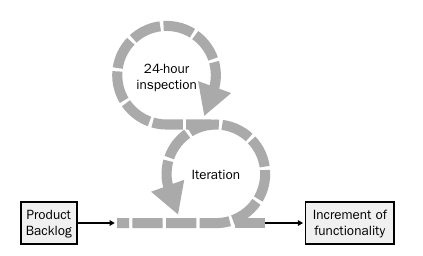
\includegraphics[scale=0.6]{images/2021-09-30_scrum_01.png}
\end{figure}


The lower circle represents an iteration of development activities that occur one after another. The output of each iteration is an increment of product. The upper circle represents the daily inspection that occurs during the iteration, in which the individual team members meet to inspect each others’ activities and make appropriate adaptations. Driving the iteration is a list of requirements. This cycle repeats until the project is no longer funded.

The skeleton operates this way: At the start of an iteration, the team reviews what it must do. It then selects what it believes it can turn into an increment of potentially shippable functionality by the end of the iteration. The team is then left alone to make its best effort for the rest of the iteration. At the end of the iteration, the team presents the increment of functionality it built so that the stakeholders can inspect the functionality and timely adaptations to the project can be made. The heart of Scrum lies in the iteration. The team takes a look at the requirements, considers the available technology, and evaluates its own skills and capabilities. It then collectively determines how to build the functionality, modifying its approach daily as it encounters new complexities, difficulties, and surprises. The team figures out what needs to be done and selects the best way to do it. This creative process is the heart of the Scrum’s productivity. Scrum implements this iterative, incremental skeleton through three roles. 

\subsection{Scrum Roles}

There are only three Scrum roles: the Product Owner, the Team, and the Scrum-Master. All management responsibilities in a project are divided among these three roles. The Product Owner is responsible for representing the interests of everyone with a stake in the project and its resulting system. The Product Owner achieves initial and ongoing funding for the project by creating the project’s initial overall requirements, return on investment (ROI) objectives, and release plans. The list of requirements is called the Product Backlog. The Product Owner is responsible for using the Product Backlog to ensure that the most valuable functionality is produced first and built upon; this is achieved by frequently prioritizing the Product Backlog to queue up the most valuable requirements for the next iteration. The Team is responsible for developing functionality. Teams are self-managing, self-organizing, and cross-functional, and they are responsible for figuring out how to turn Product Backlog into an increment of functionality within an iteration and managing their own work to do so. Team members are collectively responsible for the success of each iteraction and of the project as a whole. The ScrumMaster is responsible for the Scrum process, for teaching Scrum to everyone involved in the project, for implementing Scrum so that it fits within an organization’s culture and still delivers the expected benefits, and for ensuring that everyone follows Scrum rules and practices. The people who fill these roles are those who have committed to the project. Others might be interested in the project, but they aren’t on the hook.

Scrum makes a clear distinction between these two groups and ensures that those who are responsible for the project have the authority to do what is necessary for its success and that those who aren’t responsible can’t interfere unnecesarily. Throughout this book, I refer to these people as “pigs” and “chickens,” respectively. These names come from an old joke: A chicken and a pig are walking down the road. The chicken says to the pig, “Do you want to open a restaurant with me?” The pig considers the question and replies, “Yes, I’d like that. What do you want to call the restaurant?” The chicken replies, “Ham and Eggs!” The pig stops, pauses, and replies, “On second thought, I don’t think I want to open a restaurant with you. I’d be committed, but you’d only be involved.”

This distinction is important in Scrum and is relevant to Scrum’s insistence upon total visibility. It should always be clear who is on the hook and who is just a kibitzer. Who is responsible for the ROI, and who has a stake in the ROI but isn’t accountable? Who has to turn difficult technology into functionality, and who is a troublesome “devil’s advocate”? The rules of Scrum distinguish between the chickens and the pigs to increase productivity, create momentum, and put an end to floundering.


\subsection{Scrum Flow}

A Scrum project starts with a vision of the system to be developed. The vision might be vague at first, perhaps stated in market terms rather than system terms, but it will become clearer as the project moves forward. The Product Owner is responsible to those funding the project for delivering the vision in a manner that maximizes their ROI. The Product Owner formulates a plan for doing so that includes a Product Backlog. The Product Backlog is a list of functional and nonfunctional requirements that, when turned into functionality, will deliver this vision. The Product Backlog is prioritized so that the items most likely to generate value are top priority and is divided into proposed releases. The prioritized Product Backlog is a starting point, and the contents, priorities, and grouping of the Product Backlog into releases usually changes the moment the project starts — as should be expected. Changes in the Product Backlog reflect changing business requirements and how quickly or slowly the Team can transform Product Backlog into functionality.


All work is done in Sprints. Each Sprint is an iteration of 30 consecutive calendar days. Each Sprint is initiated with a Sprint planning meeting, where the Product Owner and Team get together to collaborate about what will be done for the next Sprint. Selecting from the highest priority Product Backlog, the Product Owner tells the Team what is desired, and the Team tells the Product Owner how much of what is desired it believes it can turn into functionality over the next Sprint. Sprint planning meetings cannot last longer than eight hours — that is, they are time-boxed to avoid too much hand-wringing about what is possible. The goal is to get to work, not to think about working. The Sprint planning meeting has two parts. The first four hours are spent with the Product Owner presenting the highest priority Product Backlog to the Team. The Team questions him or her about the content, purpose, meaning, and intentions of the Product Backlog. When the Team knows enough, but before the first four hours elapses, the Team selects as much Product Backlog as it believes it can turn into a completed increment of potentially shippable product functionality by the end of the Sprint. The Team commits to the Product Owner that it will do its best. During the second four hours of the Sprint plan- ning meeting, the Team plans out the Sprint. Because the Team is responsible for managing its own work, it needs a tentative plan to start the Sprint. The tasks that compose this plan are placed in a Sprint Backlog; the tasks in the Sprint Backlog emerge as the Sprint evolves. At the start of the second four- hour period of the Sprint planning meeting, the Sprint has started, and the clock is ticking toward the 30-day Sprint time-box. Every day, the team gets together for a 15-minute meeting called a Daily Scrum. At the Daily Scrum, each Team member answers three questions: What have you done on this project since the last Daily Scrum meeting? What do you plan on doing on this project between now and the next Daily Scrum meeting? What impediments stand in the way of you meeting your commitments to this Sprint and this project? The purpose of the meeting is to synchronize the work of all Team members daily and to schedule any meetings that the Team needs to forward its progress.

At the end of the Sprint, a Sprint review meeting is held. This is a four-hour, time-boxed meeting at which the Team presents what was developed during the Sprint to the Product Owner and any other stakeholders who want to attend. This informal meeting at which the functionality is presented is intended to bring people together and help them collaboratively determined what the Team should do next. After the Sprint review and prior to the next Sprint planning meeting, the ScrumMaster holds a Sprint retrospective meeting with the Team. At this three-hour, time-boxed meeting, the ScrumMaster encourages the Team to revise, within the Scrum process framework and practices, its development pro- cess to make it more effective and enjoyable for the next Sprint. Together, the Sprint planning meeting, the Daily Scrum, the Sprint review, and the Sprint ret- rospective constitute the empirical inspection and adaptation practices of Scrum.


\begin{figure}[H]
    \centering
    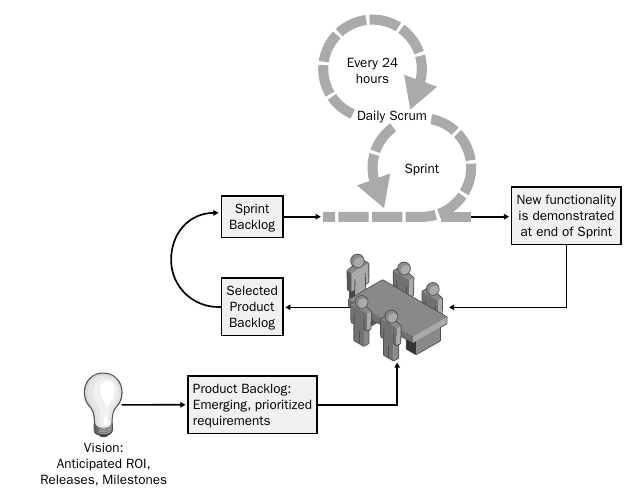
\includegraphics[scale=0.6]{images/2021-09-30_scrum_02.png}
\end{figure}


\subsection{The ScrumMaster}

The sales and marketing departments are often at odds with the development organization. Sales and marketing want quick responses to every opportunity that comes knocking. Developers need to focus on producing the product. The chaos in a company is often caused by an inability to resolve these conflicting needs. Scrum strikes a balance between the two through the use of 30-day Sprints. The development organization will do whatever is needed every Sprint, addressing whatever is deemed the top priority for that Sprint. However, everyone else must leave the developers alone to work.

The ScrumMaster is responsible for making sure that all the pieces of the Scrum process come together and work as a whole. The Product Owner must do his or her job. The Team must do its job. The chickens must be kept in line. The Product Owner and the Team must collaborate appropriately and use the Scrum meetings for inspection and adaptation. The responsibilities of the ScrumMasters can be summarized as follows:

\begin{itemize}
	\item Remove the barriers between development and the Product Owner so that the Product Owner directly drives development.
	\item Teach the Product Owner how to maximize ROI and meet his or her objectives through Scrum.
	\item Improve the lives of the development team by facilitating creativity and empowerment.
	\item Improve the productivity of the development team in any way possible.
	\item Improve the engineering practices and tools so that each increment of functionality is potentially shippable.
	\item Keep information about the team’s progress up-to-date and visible to all parties.
\end{itemize}

When the ScrumMaster fulfills these responsibilities, the project usually stays on track. These responsibilities should be enough to keep the ScrumMaster busy; no ScrumMaster should have any time left over to act like a typical boss. Indeed, a ScrumMaster who acts like a program manager probably isn’t fulfilling all of his or her duties as a ScrumMaster.


\subsection{The Product Owner}

The Product Owner is responsible for the ROI of the project, which usually means that the Product Owner chooses to develop product functionality that solves critical business problems. This is done by sorting priorities in the Product Backlog to reflect requirements with the highest business value. Traditionally, customers get to state the requirements that optimize their ROI at the start of the project, but they don’t get to assess the accuracy of their predictions until the project is completed. Scrum lets the Product Owner adjust the ROI much more frequently. 


One of the ingredients of Scrum is a practice known as sashimi. Sashimi is a Japanese delicacy consisting of thin slices of raw fish. Each slice is complete in itself, a complete taste similar to the way every other slice tastes. Scrum uses the sashimi technique to require that every slice of functionality created by the developers be complete. All of the requirements gathering and analysis, design work, coding, testing, and documentation that constitute a complete product are required to be completed in every Sprint and demonstrated in the Sprint increment of functionality. Sprints are kept short enough that the stakeholders don’t lose interest in the project before the Sprints are completed. And stakeholders can see that they have an opportunity to redirect the project at the start of every Sprint to optimize the value they derive from the project. At the end of every Sprint, stakeholders see new functionality. Models, requirements, and internal artifacts might be of use to the developers, but they are never shown to the stakeholders.


Stakeholders tend to be skeptical when first told about Scrum. Customers have had so many “silver bullets” imposed on them that they can be forgiven for this, especially since each of the silver bullets involved more work for them but fewer results. A primary tool the ScrumMaster can use to improve customer involvement is the delivery of quick results that customers can potentially use in their organization. The Sprint planning and Sprint review meetings are the bookends to initiate and fulfill this expectation. If the Team is at all capable and the project is technologically feasible, the stakeholders and Product Owner can’t wait to collaborate more with the Team.


\subsection{The Team}

Scrum’s productivity stems from doing the right things first and doing those things very effectively. The Product Owner queues up the right work by prioritizing the Product Backlog. How does the Team maximize its productivity, though? Assuming that lines of code per day or function points per person-month are good productivity measurements, who tells the Team how to maximize them?

In Scrum, the Team figures out how to maximize its productivity itself; the job of planning and executing the work belongs solely to the Team. The ScrumMaster and others can guide, advise, and inform the Team, but it is the Team’s responsi- bility to manage itself. At the heart of the solution is the Team working without interruption for the 30-day Sprint. Having selected the Product Backlog for a Sprint, the Team has mutually committed to turning it into an increment of potentially shippable product increment in 30 calendar days. Once the Team makes this commitment, the clock starts ticking. The Sprint is a time-box within which the Team does whatever is necessary to meet its commitment. At the end of the Sprint, the Team demonstrates the working functionality to the Product Owner.

As organizations implement Scrum, epiphanies are experienced, moments when people say, “Aha! Now I get it.” One such epiphany is when a Team realizes that it manages itself. The first glimpse comes during the Sprint planning meeting. The Team has selected the Product Backlog for the next Sprint—what now? The silence lengthens as the Team waits for someone to tell it what to do. The discomfort grows; when will someone step in and describe the work to the Team? At this point, I remind the Team that the Sprint has started, that there are now only 29.98 days left before the Sprint review meeting, and that no one is going to tell it what to do; the Team has to figure out its work itself. After a few more minutes, a team member speaks up, “Why don’t we figure out what the portlets should look like?” Another team member chimes in, “Do we have any standards for portlet look and feel?” The Team is now on its way. It has started to manage itself, to realize that only it can figure out the best way to reduce the Product Backlog to the demonstrable functionality.

The transition from a Team that is managed to a Team that manages itself is difficult, but the payback in productivity and pleasure of work is impressive. The ScrumMaster’s job is to lead the Team through this transition. The Scrum- Master coaches the Team to use the inspection and adaptation of the Daily Scrum to guide itself, the visibility aspects of Scrum to guide the required quality of its work, and the Sprint retrospective meeting to reflect and adapt again and again. The purpose of the Sprint retrospective is to inspect how the Scrum process worked during the last Sprint and adjust it to improve the next Sprint. These meetings are time-boxed at two hours.








%%% Local Variables:
%%% mode: latex
%%% TeX-master: "journal"
%%% End:
